

%% Dokumenttyp für Checkups / Kompetenzchecks

%%%%%%%%%%%%%%%%%%%%%%%%%%%%%%%%
%           Optionen           %
%%%%%%%%%%%%%%%%%%%%%%%%%%%%%%%%
\pgfkeys{
	/absetup/.cd,
}

%% Ggf. wurde schon als Option ein eigener Typname gesetzt
\ab@typnameSetzen{Checkup}

%%%%%%%%%%%%%%%%%%%%%%%%%%%%%%%%
%            Pakete            %
%%%%%%%%%%%%%%%%%%%%%%%%%%%%%%%%
\ab@modul@laden{tabellen}
\ab@modul@laden{icons}

%%%%%%%%%%%%%%%%%%%%%%%%%%%%%%%%
%            Makros            %
%%%%%%%%%%%%%%%%%%%%%%%%%%%%%%%%

\newcommand{\CheckupTitel}{{\usekomafont{title}Checkup\ifdefempty{\ab@titel}{}{ \Titel}\ifdefempty{\ab@reihe}{}{: \usekomafont{reihe}\Reihe}}}
\newcommand{\CheckupBild}{%
	\begin{wrapfigure}{R}{2cm}
		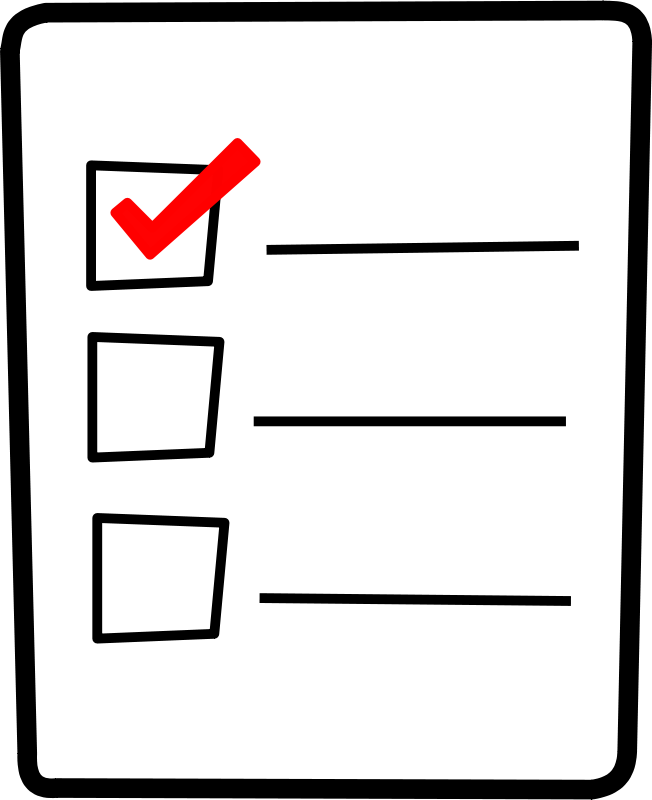
\includegraphics[width=2cm]{checkup.png}
	\end{wrapfigure}%
}

\renewcommand{\arraystretch}{1.3}

\newenvironment{checkup}{\begin{longtable}{|p{8cm}|c|p{5cm}|} \hline
	\rowcolor{ab.tabelle.kopf.hg}
	\rmfamily\textbf{Ich kann ...}
	&
	& \rmfamily\textbf{Informationen \&\newline Aufgaben} \tabularnewline \hline\hline\endhead}{\end{longtable}}

\def\ichkann#1#2{\dots #1 & \iconSkala & %
\bgroup\def\arraystretch{1}\begin{tabular}{l}
	#2
\end{tabular}\egroup \tabularnewline \hline}

%\gdef\doand{&}

% https://tex.stackexchange.com/questions/4386/defining-starred-versions-of-commands-macro
% und
% https://tex.stackexchange.com/questions/376375/using-ifstar-to-define-a-star-variant
\def\ichkannmulti{\@ifstar\@ichkannmulti\@@ichkannmulti}
\def\@ichkannmulti#1#2#3{\dots #2 & \iconSkala & \multirow{#1}{*}{#3} \tabularnewline \hline}
\def\@@ichkannmulti#1{\dots #1 & \iconSkala & \tabularnewline \cline{1-2}}

\newcommand{\teiler}[1]{\multicolumn{3}{||l||}{\color{gray}\sffamily\bfseries #1} \tabularnewline \hline}
